\documentclass[conference]{IEEEtran}
\IEEEoverridecommandlockouts

% -------------------------------------------------------
% Packages
% -------------------------------------------------------
\usepackage{cite}
\usepackage{amsmath,amssymb,amsfonts}
\usepackage{algorithmic}
\usepackage{algorithm}
\usepackage{graphicx}
\usepackage{textcomp}
\usepackage{xcolor}
\usepackage{booktabs}
\usepackage{multirow}
\usepackage{url}
\usepackage{tikz}
\usetikzlibrary{positioning,fit,calc}
\usepackage{pgfplots}
\usepackage{pgfplotstable}
\pgfplotsset{compat=1.17}
\usepgfplotslibrary{groupplots}
% Shared pgfplots styles. Colours: validated categorical palette (CVD-safe);
% each series also has a distinct dash pattern / marker for grayscale print.

\definecolor{cA}{HTML}{2A78D6} % HALX
\definecolor{cB}{HTML}{EB6834} % XGBoost
\definecolor{cC}{HTML}{1BAF7A} % RF / UNSW
\definecolor{cD}{HTML}{6250D6} % Transformer
\definecolor{cGrid}{HTML}{E4E3DF}
\pgfplotsset{
  halxbase/.style={
    tick label style={font=\tiny}, label style={font=\scriptsize},
    title style={font=\scriptsize, yshift=-1.2ex},
    legend style={font=\tiny, draw=none, fill=none},
    grid=major, major grid style={cGrid, thin},
    axis line style={black!60}, tick style={black!60},
  },
  sHALX/.style={cA, line width=1.1pt},
  sXGB/.style={cB, line width=0.9pt, densely dashed},
  sRF/.style={cC, line width=0.9pt, dash dot},
  sTR/.style={cD, line width=0.9pt, densely dotted},
}

\usepackage[hidelinks]{hyperref}

\def\BibTeX{{\rm B\kern-.05em{\sc i\kern-.025em b}\kern-.08em
    T\kern-.1667em\lower.7ex\hbox{E}\kern-.125emX}}

% auto-generated by experiments/make_report.py -- do not edit
\newcommand{\cicIsolationForestacc}{77.22}
\newcommand{\cicIsolationForestaccsd}{0.21}
\newcommand{\cicIsolationForestprec}{74.00}
\newcommand{\cicIsolationForestprecsd}{0.25}
\newcommand{\cicIsolationForestrec}{95.51}
\newcommand{\cicIsolationForestrecsd}{0.27}
\newcommand{\cicIsolationForestfOne}{83.39}
\newcommand{\cicIsolationForestfOnesd}{0.13}
\newcommand{\cicIsolationForestfpr}{50.09}
\newcommand{\cicIsolationForestfprsd}{0.73}
\newcommand{\cicIsolationForestauc}{80.64}
\newcommand{\cicIsolationForestaucsd}{0.86}
\newcommand{\cicIsolationForesttime}{0.0}
\newcommand{\cicRFacc}{99.48}
\newcommand{\cicRFaccsd}{0.08}
\newcommand{\cicRFprec}{99.59}
\newcommand{\cicRFprecsd}{0.03}
\newcommand{\cicRFrec}{99.55}
\newcommand{\cicRFrecsd}{0.11}
\newcommand{\cicRFfOne}{99.57}
\newcommand{\cicRFfOnesd}{0.07}
\newcommand{\cicRFfpr}{0.62}
\newcommand{\cicRFfprsd}{0.04}
\newcommand{\cicRFauc}{99.88}
\newcommand{\cicRFaucsd}{0.03}
\newcommand{\cicRFmfOne}{97.73}
\newcommand{\cicRFmfOnesd}{0.10}
\newcommand{\cicRFtime}{0.3}
\newcommand{\cicXGBoostacc}{99.62}
\newcommand{\cicXGBoostaccsd}{0.08}
\newcommand{\cicXGBoostprec}{99.63}
\newcommand{\cicXGBoostprecsd}{0.08}
\newcommand{\cicXGBoostrec}{99.74}
\newcommand{\cicXGBoostrecsd}{0.06}
\newcommand{\cicXGBoostfOne}{99.68}
\newcommand{\cicXGBoostfOnesd}{0.06}
\newcommand{\cicXGBoostfpr}{0.56}
\newcommand{\cicXGBoostfprsd}{0.13}
\newcommand{\cicXGBoostauc}{99.96}
\newcommand{\cicXGBoostaucsd}{0.01}
\newcommand{\cicXGBoostmfOne}{97.35}
\newcommand{\cicXGBoostmfOnesd}{0.98}
\newcommand{\cicXGBoosttime}{0.2}
\newcommand{\cicMLPacc}{97.74}
\newcommand{\cicMLPaccsd}{0.22}
\newcommand{\cicMLPprec}{97.15}
\newcommand{\cicMLPprecsd}{0.38}
\newcommand{\cicMLPrec}{99.13}
\newcommand{\cicMLPrecsd}{0.23}
\newcommand{\cicMLPfOne}{98.13}
\newcommand{\cicMLPfOnesd}{0.18}
\newcommand{\cicMLPfpr}{4.34}
\newcommand{\cicMLPfprsd}{0.60}
\newcommand{\cicMLPauc}{99.77}
\newcommand{\cicMLPaucsd}{0.01}
\newcommand{\cicMLPmfOne}{93.29}
\newcommand{\cicMLPmfOnesd}{0.43}
\newcommand{\cicMLPtime}{0.1}
\newcommand{\cicCNNLSTMacc}{97.64}
\newcommand{\cicCNNLSTMaccsd}{0.19}
\newcommand{\cicCNNLSTMprec}{97.45}
\newcommand{\cicCNNLSTMprecsd}{0.25}
\newcommand{\cicCNNLSTMrec}{98.64}
\newcommand{\cicCNNLSTMrecsd}{0.32}
\newcommand{\cicCNNLSTMfOne}{98.04}
\newcommand{\cicCNNLSTMfOnesd}{0.16}
\newcommand{\cicCNNLSTMfpr}{3.86}
\newcommand{\cicCNNLSTMfprsd}{0.40}
\newcommand{\cicCNNLSTMauc}{99.57}
\newcommand{\cicCNNLSTMaucsd}{0.05}
\newcommand{\cicCNNLSTMmfOne}{89.33}
\newcommand{\cicCNNLSTMmfOnesd}{1.58}
\newcommand{\cicCNNLSTMtime}{2.1}
\newcommand{\cicLSTMacc}{94.76}
\newcommand{\cicLSTMaccsd}{0.65}
\newcommand{\cicLSTMprec}{94.86}
\newcommand{\cicLSTMprecsd}{0.24}
\newcommand{\cicLSTMrec}{96.47}
\newcommand{\cicLSTMrecsd}{0.90}
\newcommand{\cicLSTMfOne}{95.66}
\newcommand{\cicLSTMfOnesd}{0.55}
\newcommand{\cicLSTMfpr}{7.80}
\newcommand{\cicLSTMfprsd}{0.33}
\newcommand{\cicLSTMauc}{98.88}
\newcommand{\cicLSTMaucsd}{0.14}
\newcommand{\cicLSTMmfOne}{85.40}
\newcommand{\cicLSTMmfOnesd}{3.19}
\newcommand{\cicLSTMtime}{3.7}
\newcommand{\cicTransformeracc}{98.97}
\newcommand{\cicTransformeraccsd}{0.27}
\newcommand{\cicTransformerprec}{98.82}
\newcommand{\cicTransformerprecsd}{0.34}
\newcommand{\cicTransformerrec}{99.48}
\newcommand{\cicTransformerrecsd}{0.12}
\newcommand{\cicTransformerfOne}{99.15}
\newcommand{\cicTransformerfOnesd}{0.23}
\newcommand{\cicTransformerfpr}{1.78}
\newcommand{\cicTransformerfprsd}{0.51}
\newcommand{\cicTransformerauc}{99.86}
\newcommand{\cicTransformeraucsd}{0.07}
\newcommand{\cicTransformermfOne}{95.29}
\newcommand{\cicTransformermfOnesd}{0.82}
\newcommand{\cicTransformertime}{10.6}
\newcommand{\cicHALXacc}{99.50}
\newcommand{\cicHALXaccsd}{0.09}
\newcommand{\cicHALXprec}{99.48}
\newcommand{\cicHALXprecsd}{0.07}
\newcommand{\cicHALXrec}{99.68}
\newcommand{\cicHALXrecsd}{0.08}
\newcommand{\cicHALXfOne}{99.58}
\newcommand{\cicHALXfOnesd}{0.07}
\newcommand{\cicHALXfpr}{0.77}
\newcommand{\cicHALXfprsd}{0.11}
\newcommand{\cicHALXauc}{99.95}
\newcommand{\cicHALXaucsd}{0.01}
\newcommand{\cicHALXmfOne}{95.86}
\newcommand{\cicHALXmfOnesd}{0.44}
\newcommand{\cicHALXtime}{11.0}
\newcommand{\cicablfullfOne}{99.54}
\newcommand{\cicablfullfpr}{0.84}
\newcommand{\cicablfullmfOne}{95.98}
\newcommand{\cicablnoattentionfOne}{99.58}
\newcommand{\cicablnoattentionfpr}{0.75}
\newcommand{\cicablnoattentionmfOne}{96.89}
\newcommand{\cicablnoxgboostfOne}{97.07}
\newcommand{\cicablnoxgboostfpr}{6.86}
\newcommand{\cicablnoxgboostmfOne}{90.37}
\newcommand{\cicablnorawfeaturesfOne}{99.37}
\newcommand{\cicablnorawfeaturesfpr}{1.16}
\newcommand{\cicablnorawfeaturesmfOne}{94.01}
\newcommand{\cicablnosmotefOne}{99.59}
\newcommand{\cicablnosmotefpr}{0.78}
\newcommand{\cicablnosmotemfOne}{96.78}
\newcommand{\cicablnoprivacyfOne}{99.72}
\newcommand{\cicablnoprivacyfpr}{0.65}
\newcommand{\cicablnoprivacymfOne}{94.84}
\newcommand{\cicabllstmonlyfOne}{97.07}
\newcommand{\cicabllstmonlyfpr}{5.87}
\newcommand{\cicabllstmonlymfOne}{87.96}
\newcommand{\unswIsolationForestacc}{73.24}
\newcommand{\unswIsolationForestaccsd}{0.69}
\newcommand{\unswIsolationForestprec}{69.27}
\newcommand{\unswIsolationForestprecsd}{1.58}
\newcommand{\unswIsolationForestrec}{92.73}
\newcommand{\unswIsolationForestrecsd}{3.45}
\newcommand{\unswIsolationForestfOne}{79.23}
\newcommand{\unswIsolationForestfOnesd}{0.19}
\newcommand{\unswIsolationForestfpr}{50.64}
\newcommand{\unswIsolationForestfprsd}{5.75}
\newcommand{\unswIsolationForestauc}{81.53}
\newcommand{\unswIsolationForestaucsd}{0.47}
\newcommand{\unswIsolationForesttime}{0.1}
\newcommand{\unswRFacc}{86.67}
\newcommand{\unswRFaccsd}{0.09}
\newcommand{\unswRFprec}{81.18}
\newcommand{\unswRFprecsd}{0.10}
\newcommand{\unswRFrec}{98.66}
\newcommand{\unswRFrecsd}{0.06}
\newcommand{\unswRFfOne}{89.07}
\newcommand{\unswRFfOnesd}{0.07}
\newcommand{\unswRFfpr}{28.03}
\newcommand{\unswRFfprsd}{0.20}
\newcommand{\unswRFauc}{97.86}
\newcommand{\unswRFaucsd}{0.02}
\newcommand{\unswRFmfOne}{49.04}
\newcommand{\unswRFmfOnesd}{0.31}
\newcommand{\unswRFtime}{1.3}
\newcommand{\unswXGBoostacc}{86.81}
\newcommand{\unswXGBoostaccsd}{0.14}
\newcommand{\unswXGBoostprec}{81.57}
\newcommand{\unswXGBoostprecsd}{0.18}
\newcommand{\unswXGBoostrec}{98.22}
\newcommand{\unswXGBoostrecsd}{0.02}
\newcommand{\unswXGBoostfOne}{89.13}
\newcommand{\unswXGBoostfOnesd}{0.10}
\newcommand{\unswXGBoostfpr}{27.18}
\newcommand{\unswXGBoostfprsd}{0.33}
\newcommand{\unswXGBoostauc}{98.26}
\newcommand{\unswXGBoostaucsd}{0.03}
\newcommand{\unswXGBoostmfOne}{49.93}
\newcommand{\unswXGBoostmfOnesd}{0.84}
\newcommand{\unswXGBoosttime}{1.2}
\newcommand{\unswMLPacc}{86.36}
\newcommand{\unswMLPaccsd}{0.24}
\newcommand{\unswMLPprec}{81.39}
\newcommand{\unswMLPprecsd}{1.00}
\newcommand{\unswMLPrec}{97.57}
\newcommand{\unswMLPrecsd}{1.32}
\newcommand{\unswMLPfOne}{88.73}
\newcommand{\unswMLPfOnesd}{0.05}
\newcommand{\unswMLPfpr}{27.38}
\newcommand{\unswMLPfprsd}{2.15}
\newcommand{\unswMLPauc}{97.75}
\newcommand{\unswMLPaucsd}{0.49}
\newcommand{\unswMLPmfOne}{43.70}
\newcommand{\unswMLPmfOnesd}{1.38}
\newcommand{\unswMLPtime}{0.2}
\newcommand{\unswCNNLSTMacc}{86.13}
\newcommand{\unswCNNLSTMaccsd}{0.35}
\newcommand{\unswCNNLSTMprec}{80.63}
\newcommand{\unswCNNLSTMprecsd}{0.42}
\newcommand{\unswCNNLSTMrec}{98.47}
\newcommand{\unswCNNLSTMrecsd}{0.38}
\newcommand{\unswCNNLSTMfOne}{88.66}
\newcommand{\unswCNNLSTMfOnesd}{0.26}
\newcommand{\unswCNNLSTMfpr}{28.98}
\newcommand{\unswCNNLSTMfprsd}{0.82}
\newcommand{\unswCNNLSTMauc}{98.17}
\newcommand{\unswCNNLSTMaucsd}{0.10}
\newcommand{\unswCNNLSTMmfOne}{42.43}
\newcommand{\unswCNNLSTMmfOnesd}{0.35}
\newcommand{\unswCNNLSTMtime}{2.1}
\newcommand{\unswLSTMacc}{84.99}
\newcommand{\unswLSTMaccsd}{0.05}
\newcommand{\unswLSTMprec}{79.25}
\newcommand{\unswLSTMprecsd}{0.24}
\newcommand{\unswLSTMrec}{98.54}
\newcommand{\unswLSTMrecsd}{0.39}
\newcommand{\unswLSTMfOne}{87.85}
\newcommand{\unswLSTMfOnesd}{0.01}
\newcommand{\unswLSTMfpr}{31.61}
\newcommand{\unswLSTMfprsd}{0.58}
\newcommand{\unswLSTMauc}{97.94}
\newcommand{\unswLSTMaucsd}{0.13}
\newcommand{\unswLSTMmfOne}{40.76}
\newcommand{\unswLSTMmfOnesd}{0.88}
\newcommand{\unswLSTMtime}{4.5}
\newcommand{\unswTransformeracc}{86.94}
\newcommand{\unswTransformeraccsd}{2.60}
\newcommand{\unswTransformerprec}{82.28}
\newcommand{\unswTransformerprecsd}{3.89}
\newcommand{\unswTransformerrec}{97.66}
\newcommand{\unswTransformerrecsd}{1.48}
\newcommand{\unswTransformerfOne}{89.23}
\newcommand{\unswTransformerfOnesd}{1.78}
\newcommand{\unswTransformerfpr}{26.18}
\newcommand{\unswTransformerfprsd}{7.31}
\newcommand{\unswTransformerauc}{98.09}
\newcommand{\unswTransformeraucsd}{0.29}
\newcommand{\unswTransformermfOne}{43.69}
\newcommand{\unswTransformermfOnesd}{1.49}
\newcommand{\unswTransformertime}{12.2}
\newcommand{\unswHALXacc}{86.78}
\newcommand{\unswHALXaccsd}{0.08}
\newcommand{\unswHALXprec}{81.56}
\newcommand{\unswHALXprecsd}{0.07}
\newcommand{\unswHALXrec}{98.20}
\newcommand{\unswHALXrecsd}{0.13}
\newcommand{\unswHALXfOne}{89.11}
\newcommand{\unswHALXfOnesd}{0.07}
\newcommand{\unswHALXfpr}{27.21}
\newcommand{\unswHALXfprsd}{0.14}
\newcommand{\unswHALXauc}{98.25}
\newcommand{\unswHALXaucsd}{0.05}
\newcommand{\unswHALXmfOne}{48.27}
\newcommand{\unswHALXmfOnesd}{0.50}
\newcommand{\unswHALXtime}{13.9}
\newcommand{\unswablfullfOne}{89.20}
\newcommand{\unswablfullfpr}{27.22}
\newcommand{\unswablfullmfOne}{47.70}
\newcommand{\unswablnoattentionfOne}{88.89}
\newcommand{\unswablnoattentionfpr}{27.38}
\newcommand{\unswablnoattentionmfOne}{48.44}
\newcommand{\unswablnoxgboostfOne}{88.96}
\newcommand{\unswablnoxgboostfpr}{27.34}
\newcommand{\unswablnoxgboostmfOne}{41.87}
\newcommand{\unswablnorawfeaturesfOne}{88.93}
\newcommand{\unswablnorawfeaturesfpr}{27.13}
\newcommand{\unswablnorawfeaturesmfOne}{45.01}
\newcommand{\unswablnosmotefOne}{89.22}
\newcommand{\unswablnosmotefpr}{26.62}
\newcommand{\unswablnosmotemfOne}{48.09}
\newcommand{\unswablnoprivacyfOne}{89.17}
\newcommand{\unswablnoprivacyfpr}{26.89}
\newcommand{\unswablnoprivacymfOne}{49.15}
\newcommand{\unswabllstmonlyfOne}{87.50}
\newcommand{\unswabllstmonlyfpr}{33.13}
\newcommand{\unswabllstmonlymfOne}{39.82}
\newcommand{\unswthru}{4{,}885}
\newcommand{\unswlatmed}{3.74}
\newcommand{\unswlatpn}{4.88}
\newcommand{\unswprivus}{0.73}
\newcommand{\unswparams}{61{,}690}
\newcommand{\cicthru}{3{,}899}
\newcommand{\ciclatmed}{3.19}
\newcommand{\ciclatpn}{4.81}
\newcommand{\cicprivus}{0.62}
\newcommand{\cicparams}{61{,}255}
\newcommand{\cicfpsharelowmedium}{69.2}
\newcommand{\cicalertsharehigh}{98.4}
\newcommand{\cictopOneZeroattackmass}{41.9}
\newcommand{\cicsevlow}{56.7}
\newcommand{\cicsevnlow}{30}
\newcommand{\cicsevmedium}{90.4}
\newcommand{\cicsevnmedium}{52}
\newcommand{\cicsevhigh}{99.8}
\newcommand{\cicsevnhigh}{5{,}020}
\newcommand{\cicsevbenign}{0.4}
\newcommand{\cicsevnbenign}{3{,}398}
\newcommand{\unswfpsharelowmedium}{87.3}
\newcommand{\unswalertsharehigh}{77.1}
\newcommand{\unswtopOneZeroattackmass}{57.8}
\newcommand{\unswsevlow}{22.8}
\newcommand{\unswsevnlow}{6{,}813}
\newcommand{\unswsevmedium}{38.2}
\newcommand{\unswsevnmedium}{5{,}702}
\newcommand{\unswsevhigh}{97.0}
\newcommand{\unswsevnhigh}{42{,}156}
\newcommand{\unswsevbenign}{2.6}
\newcommand{\unswsevnbenign}{27{,}661}
\newcommand{\PRIVCOSTMAX}{0.11}
\newcommand{\cicgapfOne}{3.9}
\newcommand{\cicfprratio}{10}
\newcommand{\cicprivcost}{0.11}
\newcommand{\cicIsolationForesttprOne}{1.1}
\newcommand{\cicRFtprOne}{99.6}
\newcommand{\cicXGBoosttprOne}{99.8}
\newcommand{\cicMLPtprOne}{94.6}
\newcommand{\cicCNNLSTMtprOne}{94.2}
\newcommand{\cicLSTMtprOne}{80.4}
\newcommand{\cicTransformertprOne}{99.0}
\newcommand{\cicHALXtprOne}{99.8}
\newcommand{\unswgapfOne}{1.3}
\newcommand{\unswfprratio}{1}
\newcommand{\unswprivcost}{-0.03}
\newcommand{\unswIsolationForesttprOne}{0.5}
\newcommand{\unswRFtprOne}{77.7}
\newcommand{\unswXGBoosttprOne}{85.9}
\newcommand{\unswMLPtprOne}{81.0}
\newcommand{\unswCNNLSTMtprOne}{84.9}
\newcommand{\unswLSTMtprOne}{81.9}
\newcommand{\unswTransformertprOne}{82.6}
\newcommand{\unswHALXtprOne}{86.9}

% Mean attention-pooling weight per feature token (top-10 for attack flows), test set, seed 0.
% #1 = dataset key (cic/unsw)
\begin{tikzpicture}
\begin{axis}[
  halxbase, xbar=0pt, width=0.95\columnwidth, height=0.62\columnwidth,
  bar width=2.3pt, xmin=0, xlabel={Mean attention weight $\bar\alpha_j$ (\%)},
  ytick=data, yticklabels from table={generated/attn_#1.dat}{name},
  y tick label style={font=\tiny}, enlarge y limits=0.06,
  legend style={at={(0.98,0.03)}, anchor=south east, font=\tiny},
  major y grid style={draw=none}, area legend,
]
\addplot[fill=cA, draw=none] table[y=i, x=attack] {generated/attn_#1.dat};
\addplot[fill=cB, draw=none] table[y=i, x=benign] {generated/attn_#1.dat};
\legend{attack flows, benign flows}
\end{axis}
\end{tikzpicture}

\providecommand{\ABLunswSeeds}{seed 0}
\providecommand{\ABLATIONTEXT}{[ablation text]}
\providecommand{\PRIVACYTEXT}{[privacy text]}
\providecommand{\EXPLAINTEXT}{[explain text]}
\providecommand{\COSTTEXT}{[cost text]}


\begin{document}

\title{HALX: Privacy-Preserving Hybrid Attention-LSTM and XGBoost
Framework for Proactive Threat Detection in Financial Networks}

\author{
\IEEEauthorblockN{Mubasshir Ahmed}
\IEEEauthorblockA{
\textit{Victoria University}\\
Melbourne, Australia\\
mubasshir.ahmed@live.vu.edu.au}
\and
\IEEEauthorblockN{Md Mazharul Islam}
\IEEEauthorblockA{
\textit{Electrical and Computer Engineering}\\
\textit{North South University}\\
Dhaka, Bangladesh\\
mazharul.islam1@northsouth.edu}
}

\maketitle

\begin{abstract}
Financial institutions need intrusion detectors that are accurate and
auditable and that do not themselves become a channel for leaking customer
data. We present HALX, a framework for proactive threat detection in
financial networks with three parts: a feature-token Attention-LSTM
encoder, an XGBoost scoring head, and a privacy-preserving inference layer.
The privacy layer enforces Mondrian $k$-anonymity on quasi-identifiers and
releases the preprocessing statistics under $(\varepsilon,\delta)$-differential
privacy. Every alert carries a threat score, a severity tier and the
most-attended features as an explanation. We compare HALX with seven
baselines over three seeds on the official UNSW-NB15 split and on a
CICIDS2017 subset, giving every method the same privatized inputs. On
CICIDS2017, HALX reaches an F1-score of \cicHALXfOne\% at a
\cicHALXfpr\% false-positive rate. This is on par with the strongest tree
ensembles and gives 2--10$\times$ fewer false alarms than CNN-LSTM, BiLSTM
and Transformer detectors. On UNSW-NB15, a train--test distribution shift
holds every model near 89\% F1 on average. There HALX matches XGBoost
(\unswHALXfOne\%), has the most stable false-positive rate across seeds,
and detects the most attacks at a 1\% false-alarm budget
(\unswHALXtprOne\%, seed 0). Under this shift,
\unswsevhigh\% of its high-severity alerts are real attacks. The privacy
layer ($k{=}10$, $\varepsilon{=}1$) costs at most \PRIVCOSTMAX{} F1 points,
and HALX scores thousands of flows per second on a CPU. Code and results
are publicly available.
\end{abstract}


\begin{IEEEkeywords}
Intrusion detection, financial cybersecurity, attention-LSTM, XGBoost,
$k$-anonymity, differential privacy, explainable AI, PCI~DSS, GDPR
\end{IEEEkeywords}

% ======================================================================
\section{Introduction}
% ======================================================================
Payment switches, core-banking platforms and the cloud services that host
them are prime targets. The financial sector had the second-highest
average breach cost of 17 industries in the IBM 2024 study, at
US\$6.08 million per incident~\cite{ibm2024breach}, and banks face DDoS,
ransomware, insider misuse and multi-stage
intrusions~\cite{asmar2024banks,islam2022ddosbank}. Signature-based
intrusion detection systems (IDS) miss unseen attacks, and a reactive
security operations centre (SOC) learns of an intrusion only after the damage
is done. \emph{Proactive} detection instead scores every flow as it is
observed and gives analysts a ranked, explained set of alerts.

Recent ML-based IDS use increasingly elaborate deep models: CNN--LSTM
hybrids~\cite{halbouni2022cnnlstm,altunay2023cnnlstm}, attention-augmented
recurrent networks~\cite{alashjaee2025attn} and
transformers~\cite{wu2022rtids,manocchio2024flowtransformer,akuthota2025iot}.
Deploying them in a regulated institution raises three issues that
benchmark accuracy does not capture.
\textit{(i) Tabular reality.} Flow records are tabular, where
gradient-boosted trees remain hard to beat~\cite{grinsztajn2022tree}, so a
deep detector must be compared with a tuned boosted-tree baseline. \textit{(ii) Privacy and compliance.} Flow
features such as transferred volumes, session durations and TTL or window
values act as \emph{quasi-identifiers} of customers and hosts. Under GDPR
Art.~25 (data protection by design)~\cite{gdpr2016} and PCI~DSS~\cite{pcidss4},
the detector and what it stores must not become a new leakage channel. \textit{(iii) Auditability.} Analysts need to know \emph{why} a flow
was flagged and how urgent it is~\cite{neupane2022xids}.

We present \textbf{HALX} (\underline{H}ybrid
\underline{A}ttention-\underline{L}STM + \underline{X}GBoost), which
addresses all three. Our contributions are:
\begin{itemize}
  \item A hybrid detector: a feature-token Attention-LSTM encoder learns a
        flow representation that an XGBoost head~\cite{chen2016xgboost}
        scores together with the privatized features, yielding a threat
        probability and three severity tiers.
  \item A privacy-preserving inference layer with \emph{formally stated}
        guarantees: Mondrian $k$-anonymity~\cite{lefevre2006mondrian} on
        quasi-identifiers and $(\varepsilon,\delta)$-DP preprocessing
        statistics with zCDP accounting~\cite{bun2016zcdp}.
  \item A reproducible evaluation on UNSW-NB15~\cite{moustafa2015unsw} and
        CICIDS2017~\cite{sharafaldin2018cicids} against seven baselines over
        three seeds, with ablation, privacy--utility, explanation and
        latency analyses. Code and results are released.\footnote{\url{https://github.com/mazharulmd/Threat-Detection-for-Financial-Systems}}
\end{itemize}

% ======================================================================
\section{Related Work}
\label{sec:related}
% ======================================================================
\textbf{Deep and hybrid IDS.} CNN--LSTM models combine convolutional
feature extraction with recurrent modelling and are a common baseline on
CICIDS2017 and UNSW-NB15~\cite{halbouni2022cnnlstm,altunay2023cnnlstm}.
Alashjaee~\cite{alashjaee2025attn} adds self-attention to a CNN--LSTM and
shows in an ablation that the attention layer helps.
Transformer-based detectors treat flow features as
tokens~\cite{wu2022rtids,long2024cloud,akuthota2025iot}. FlowTransformer
showed that the choice of input encoding and classification head matters more
than the transformer variant~\cite{manocchio2024flowtransformer}, and
BERT-style language models have also been adapted to
traffic~\cite{yang2025bert}. Closest to our work, Sajid et
al.~\cite{sajid2024hybrid} use XGBoost and a CNN as feature selectors in
front of an LSTM classifier. HALX reverses that order: the deep encoder
produces the representation and the boosted trees make the decision. This
follows evidence that trees are the stronger final learner on tabular
data~\cite{grinsztajn2022tree,gorishniy2021revisiting}.

\textbf{ML security in finance.} Surveys of digital banking identify DDoS,
ransomware, insider threats and phishing as the dominant threat
classes~\cite{asmar2024banks}. Islam et al.~\cite{islam2022ddosbank} detect
DDoS on a banking IoT monitoring system. Recent studies report SOC
deployments in core-banking systems~\cite{bhowmick2026cbs} and proactive
detection in emulated bank networks~\cite{mulea2026banking}. They stress
regulatory constraints, but none of them states a formal privacy guarantee
for the detector itself.

\textbf{Privacy-preserving IDS.} Most privacy work on IDS concerns
\emph{training}: federated learning~\cite{mcmahan2017fedavg} with
differentially private updates~\cite{ruzafa2023fl,gutti2025fl,vyas2024ppfl},
or DP-SGD~\cite{abadi2016dpsgd}. We address a complementary
problem that is often overlooked: what the deployed detector \emph{exposes},
namely generalized quasi-identifiers in its inputs and logs and the
normalization statistics shipped with the model. The two approaches can be
combined.

\textbf{Evaluation pitfalls.} CICIDS2017 contains labelling and flow-construction
errors~\cite{engelen2021troubleshooting}, and models trained on it transfer
poorly to related traffic~\cite{catillo2022transferability}. Arp et
al.~\cite{arp2022dos} catalogue pitfalls such as data snooping and
inappropriate baselines. We follow their recommendations: the test
partitions are never used for model selection, a tuned XGBoost baseline is
always included, and every number is reported as a mean over seeds.
Explainability is surveyed in~\cite{neupane2022xids}, and
\cite{barnard2022xai} pairs XGBoost with SHAP for NIDS. HALX instead
explains each alert through its intrinsic attention weights.

% ======================================================================
\section{Threat Model and Problem Statement}
\label{sec:problem}
% ======================================================================
We consider the network segment of a financial institution (for example
core banking, payment switching or online banking front-ends) monitored by a
flow exporter. Each bidirectional flow is summarized as a record
$\mathbf{r}=(\mathbf{r}^{\mathrm{num}},\mathbf{r}^{\mathrm{cat}})$ with $d$
numeric and $c$ categorical attributes. The adversary is an external or
insider attacker whose activity (reconnaissance, exploitation, DoS/DDoS,
brute force, botnet C\&C, web attacks, backdoors) produces flows. The task
is to output, for every flow, a threat score $p\in[0,1]$, a binary decision
$\hat{y}=\mathbb{1}[p\ge\tau]$, an attack family and a severity tier. A
second, \emph{honest-but-curious} party is also considered: an operator,
vendor or auditor who sees the detector's stored inputs and its released
preprocessing statistics. Against this party HALX must limit
re-identification of individual flows.

% ======================================================================
\section{Proposed Framework: HALX}
\label{sec:method}
% ======================================================================
Fig.~\ref{fig:architecture} shows the three stages: (1) a privacy-preserving
layer, (2) an Attention-LSTM encoder and (3) an XGBoost scoring head with
severity triage. Algorithm~\ref{alg:halx} summarizes training.

\begin{figure*}[t]
\centering
\resizebox{0.97\textwidth}{!}{% HALX architecture (TikZ). Included from main.tex.
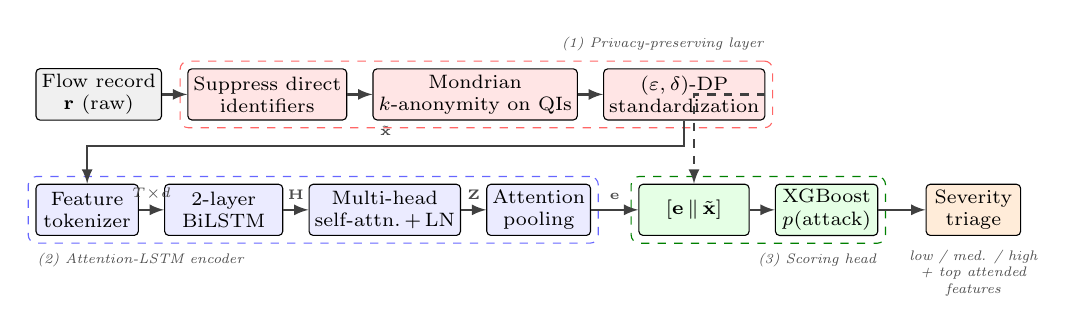
\begin{tikzpicture}[
  font=\scriptsize, >=latex, node distance=3.2mm,
  blk/.style={draw, rounded corners=1.5pt, align=center, minimum height=6.5mm, inner sep=2pt, fill=#1},
  blk/.default=white,
  grp/.style={draw, dashed, rounded corners=3pt, inner sep=2.6pt},
  lab/.style={font=\tiny\itshape, text=black!70},
  arr/.style={->, thick, black!75}]
% ---- input and privacy layer
\node[blk=gray!12, minimum width=13mm] (raw) {Flow record\\$\mathbf{r}$ (raw)};
\node[blk=red!10, right=of raw, minimum width=17mm] (sup) {Suppress direct\\identifiers};
\node[blk=red!10, right=of sup, minimum width=19mm] (mond) {Mondrian\\$k$-anonymity on QIs};
\node[blk=red!10, right=of mond, minimum width=16mm] (dp) {$(\varepsilon,\delta)$-DP\\standardization};
\node[grp, draw=red!60, fit=(sup)(mond)(dp), label={[lab, anchor=south east]north east:(1) Privacy-preserving layer}] (P) {};
\draw[arr] (raw) -- (sup); \draw[arr] (sup) -- (mond); \draw[arr] (mond) -- (dp);
% ---- encoder
\node[blk=blue!8, below=8mm of raw.south west, anchor=north west, minimum width=13mm] (tok) {Feature\\tokenizer};
\node[blk=blue!8, right=of tok, minimum width=15mm] (lstm) {2-layer\\BiLSTM};
\node[blk=blue!8, right=of lstm, minimum width=15mm] (mha) {Multi-head\\self-attn.\,+\,LN};
\node[blk=blue!8, right=of mha, minimum width=13mm] (pool) {Attention\\pooling};
\node[grp, draw=blue!60, fit=(tok)(lstm)(mha)(pool), label={[lab, anchor=north west]south west:(2) Attention-LSTM encoder}] (E) {};
\draw[arr] (tok) -- node[above, lab]{$T{\times}d$} (lstm);
\draw[arr] (lstm) -- node[above, lab]{$\mathbf{H}$} (mha);
\draw[arr] (mha) -- node[above, lab]{$\mathbf{Z}$} (pool);
\draw[arr] (dp.south) |- ++(0,-3.2mm) -| node[pos=0.25, above, lab]{$\tilde{\mathbf{x}}$} (tok.north);
% ---- head
\node[blk=green!10, right=6mm of pool, minimum width=14mm] (cat) {$[\mathbf{e}\,\Vert\,\tilde{\mathbf{x}}]$};
\node[blk=green!10, right=of cat, minimum width=13mm] (xgb) {XGBoost\\$p(\text{attack})$};
\node[grp, draw=green!50!black, fit=(cat)(xgb), label={[lab, anchor=north east]south east:(3) Scoring head}] (X) {};
\draw[arr] (pool) -- node[above, lab]{$\mathbf{e}$} (cat);
\draw[arr] (cat) -- (xgb);
\draw[arr, dashed] (dp.east) -| (cat.north);
% ---- alerting
\node[blk=orange!15, right=6mm of xgb, minimum width=12mm] (alert) {Severity\\triage};
\draw[arr] (xgb) -- (alert);
\node[lab, below=0.5mm of alert, align=center] {low / med. / high\\+ top attended\\features};
\end{tikzpicture}
}
\caption{The HALX pipeline. Raw flow records pass through the privacy layer
(direct-identifier suppression, Mondrian $k$-anonymous generalization of
quasi-identifiers, DP standardization). The Attention-LSTM encoder reads the
privatized record as a sequence of feature tokens and produces an embedding
$\mathbf{e}$. XGBoost scores $[\mathbf{e}\Vert\tilde{\mathbf{x}}]$, and the score is
mapped to a severity tier together with the most-attended features.}
\label{fig:architecture}
\end{figure*}

\subsection{Privacy-Preserving Layer}
\label{sec:privacy}
\textit{Suppression.} Direct identifiers (IP addresses, ports,
timestamps, flow IDs) are dropped before any processing.

\textit{Quasi-identifier generalization.} Let $Q\subset\{1,\dots,d\}$ be the
quasi-identifiers (QIs). On UNSW-NB15 these are duration, source and
destination bytes, and source TTL; on CICIDS2017 they are flow duration,
forward and backward payload lengths, and the initial forward TCP window.
Volumes play the role of transaction sizes, and TTL or window values
fingerprint operating systems. After a public, data-independent transform
$g(x)=\operatorname{sign}(x)\log(1+|x|)$, we build a strict Mondrian
partition~\cite{lefevre2006mondrian} of the training QIs. Each region is
split recursively at the median of its widest normalized QI, as long as both
children keep at least $k$ records. Every record, in training or at
inference, is routed to its leaf and its QIs are replaced by the leaf median.
Hence every generalized QI vector the detector stores or logs is shared by
at least $k$ training records ($k$-anonymity~\cite{sweeney2002kanon}). We use
$k=10$ by default and verify the smallest equivalence class after fitting.

\textit{DP standardization.} Standardization needs per-feature means and
variances, which are normally shipped with a model and can reveal individual
records when an outlier dominates. We release them with the Gaussian
mechanism. With values clipped to $[-C,C]$ ($C=25$ in $g$-space) and public
$n$, the sums $S_1=\sum_i x_i$ and $S_2=\sum_i x_i^2$ have replace-one
sensitivities $2C$ and $C^2$. Each of the $2d$ released sums receives noise
$\mathcal{N}(0,\Delta^2/2\rho_q)$ with $\rho_q=\rho/2d$, where
\begin{equation}
  \rho=\Bigl(\sqrt{\ln(1/\delta)+\varepsilon}-\sqrt{\ln(1/\delta)}\Bigr)^2
  \label{eq:rho}
\end{equation}
is the largest $\rho$ for which $\rho$-zCDP implies
$(\varepsilon,\delta)$-DP, using $\varepsilon=\rho+2\sqrt{\rho\ln(1/\delta)}$~\cite{bun2016zcdp}.
By composition, the released statistics satisfy
$(\varepsilon,\delta)$-DP. We use $\varepsilon=1$ and $\delta=10^{-5}$.
\emph{Scope:} this protects the shipped statistics only. The network
weights are not differentially private; that would require
DP-SGD~\cite{abadi2016dpsgd} (Sec.~\ref{sec:discussion}).

\subsection{Attention-LSTM Encoder}
\label{sec:encoder}
UNSW-NB15's partition files carry no timestamps and are sorted by label, and
the CICIDS2017 subset is randomly sampled. Sliding windows of
\emph{consecutive flows} would therefore leak labels through ordering, a form of
data snooping~\cite{arp2022dos}. HALX instead reads each flow record as a
sequence of $T=d+c$ \emph{feature tokens}, in the spirit of tabular
transformers~\cite{gorishniy2021revisiting}:
\begin{equation}
  \mathbf{t}_j=\tilde{x}_j\,\mathbf{w}_j+\mathbf{b}_j\ (j\le d),\qquad
  \mathbf{t}_{d+i}=\mathbf{E}_i[r^{\mathrm{cat}}_i]+\mathbf{b}_{d+i},
  \label{eq:tok}
\end{equation}
with $\mathbf{w}_j,\mathbf{b}_j\in\mathbb{R}^{16}$. A two-layer bidirectional
LSTM~\cite{hochreiter1997lstm} with 32 units per direction produces
$\mathbf{H}=[\mathbf{h}_1,\dots,\mathbf{h}_T]\in\mathbb{R}^{T\times64}$. Here
the recurrence models interactions between related features, for example
packet counts, sizes and rates of the same direction. Multi-head
self-attention~\cite{vaswani2017attention} with $H=4$ heads lets every token
attend to every other:
\begin{equation}
  \mathbf{Z}=\mathrm{LN}\bigl(\mathbf{H}+\mathrm{MHA}(\mathbf{H}\mathbf{W}^Q,
  \mathbf{H}\mathbf{W}^K,\mathbf{H}\mathbf{W}^V)\bigr),
  \label{eq:mha}
\end{equation}
where each head computes
$\mathrm{softmax}(QK^{\top}/\sqrt{d_k})V$. Additive attention pooling
then yields the flow embedding together with an importance distribution
over features:
\begin{equation}
  \alpha_j=\operatorname{softmax}_j\bigl(\mathbf{u}^{\top}\tanh(\mathbf{W}_a\mathbf{z}_j)\bigr),\qquad
  \mathbf{e}=\textstyle\sum_{j}\alpha_j\mathbf{z}_j .
  \label{eq:pool}
\end{equation}
The weights $\alpha_j$ are reported with each alert as an explanation.
The encoder is trained end to end with a linear softmax head on the
multi-class labels (cross-entropy, AdamW, learning rate $3\cdot10^{-3}$,
cosine schedule, batch 1024). Early stopping uses validation macro-F1.

\subsection{XGBoost Scoring Head and Severity Triage}
\label{sec:head}
The deep encoder captures cross-feature structure, but on tabular data
boosted trees model sharp, axis-aligned decision boundaries better~\cite{grinsztajn2022tree}.
The head therefore receives the concatenation
$\mathbf{f}=[\mathbf{e}\,\Vert\,\tilde{\mathbf{x}}]$ of the embedding and the
privatized features. One XGBoost model~\cite{chen2016xgboost} estimates
$p=P(\text{attack}\mid\mathbf{f})$ and a second predicts the attack family
(up to 800 trees, depth 8, learning rate 0.08, early stopping on the
validation split). Alerts with $p\ge\tau=0.5$ are triaged into
\emph{low} ($p<0.8$), \emph{medium} ($0.8\le p<0.95$) and \emph{high}
($p\ge0.95$) severity, so SOC analysts can work through high-severity alerts first.

\begin{algorithm}[t]
\caption{HALX training}
\label{alg:halx}
\begin{algorithmic}[1]
\REQUIRE training/validation flows $\mathcal{D}_{tr},\mathcal{D}_{va}$; QI set $Q$; $k,\varepsilon,\delta$
\STATE Drop direct identifiers; apply $g(\cdot)$; impute with training medians
\STATE Fit Mondrian tree on $\mathcal{D}_{tr}[Q]$ with leaf size $\ge k$; generalize $Q$
\STATE Release $(\mu,\sigma)$ via Gaussian mechanism with $\rho(\varepsilon,\delta)$ (Eq.~\ref{eq:rho}); standardize $\to\tilde{\mathbf{x}}$
\STATE Oversample minority families in $\mathcal{D}_{tr}$ with SMOTE-NC~\cite{chawla2002smote}
\STATE Train encoder (Eqs.~\ref{eq:tok}--\ref{eq:pool}) with early stopping on $\mathcal{D}_{va}$
\STATE Extract $\mathbf{f}=[\mathbf{e}\Vert\tilde{\mathbf{x}}]$ for $\mathcal{D}_{tr},\mathcal{D}_{va}$
\STATE Fit binary and multi-class XGBoost on $\mathcal{D}_{tr}$, early-stopped on $\mathcal{D}_{va}$
\RETURN privacy layer, encoder, XGBoost heads, threshold $\tau$
\end{algorithmic}
\end{algorithm}

% ======================================================================
\section{Implementation and Experimental Setup}
\label{sec:exp}
% ======================================================================
\subsection{Datasets and Protocol}
\textbf{UNSW-NB15}~\cite{moustafa2015unsw}: we use the official partition
(175{,}341 training / 82{,}332 test flows; 9 attack families; 39 numeric
and 3 categorical attributes, i.e.\ 42 tokens). 15\% of the training part
is held out for validation, and the test set is used only for final
reporting. Its attack share differs from training (55.1\% vs.\ 68.1\%),
which makes this the harder, more realistic setting.
\textbf{CICIDS2017}~\cite{sharafaldin2018cicids}: we use the publicly
released stratified subset of Yang et al.~\cite{yang2022mthids}
(56{,}661 flows, 77 features, 6 grouped attack classes: DoS, PortScan,
brute force, web attack, bot and infiltration; 60 informative numeric
features). We split it 70/15/15 (39{,}662/8{,}499/8{,}500 flows) with
stratification. Given known labelling issues~\cite{engelen2021troubleshooting},
we treat it as a second, easier benchmark.
Duplicate and constant columns (decided on training data only) are removed,
infinite values are imputed with training medians, and categorical
attributes keep their 31 most frequent levels plus an ``other'' bucket.
SMOTE-NC~\cite{chawla2002smote} raises every attack family to at least 2\% of
the \emph{training} split only. Every configuration is run with three seeds
(0, 1, 2); the seed changes the train/validation split, SMOTE, weight
initialization and the DP noise. We report mean${}\pm{}$std.


\subsection{Baselines}
All baselines receive the same privatized inputs:
(i) Isolation Forest~\cite{liu2008iforest}, trained on benign flows only, with
the threshold chosen on validation F1;
(ii) Random Forest~\cite{breiman2001rf} (300 trees);
(iii) XGBoost~\cite{chen2016xgboost}, configured exactly like the HALX head;
(iv) a two-layer MLP (256 units);
(v) CNN-LSTM in the style of~\cite{halbouni2022cnnlstm} (two Conv1d layers
followed by an LSTM over feature tokens);
(vi) the HALX BiLSTM without attention and without the XGBoost head; and
(vii) a feature-token Transformer (FT-Transformer style~\cite{gorishniy2021revisiting},
two layers, 4 heads, $d=64$), which stands in for the transformer IDS
family~\cite{wu2022rtids,manocchio2024flowtransformer}. The deep baselines
use the same optimizer, schedule and early-stopping rule as HALX.

\subsection{Implementation}
HALX uses PyTorch~2, XGBoost~3 and scikit-learn; the privacy layer
(Mondrian tree, zCDP standardizer) is ${\approx}150$ lines of NumPy. All
runs used a 4-core x86 CPU (16\,GB RAM, no GPU), at most 15 epochs (8 on
UNSW-NB15) and patience 3. We report accuracy, precision, recall, F1 and
FPR for the binary decision at $\tau=0.5$, ROC-AUC, and macro-F1 (M-F1)
over attack families.

% ======================================================================
\section{Results}
\label{sec:results}
% ======================================================================
% auto-generated by experiments/make_report.py -- do not edit
\newcommand{\cicIsolationForestacc}{77.22}
\newcommand{\cicIsolationForestaccsd}{0.21}
\newcommand{\cicIsolationForestprec}{74.00}
\newcommand{\cicIsolationForestprecsd}{0.25}
\newcommand{\cicIsolationForestrec}{95.51}
\newcommand{\cicIsolationForestrecsd}{0.27}
\newcommand{\cicIsolationForestfOne}{83.39}
\newcommand{\cicIsolationForestfOnesd}{0.13}
\newcommand{\cicIsolationForestfpr}{50.09}
\newcommand{\cicIsolationForestfprsd}{0.73}
\newcommand{\cicIsolationForestauc}{80.64}
\newcommand{\cicIsolationForestaucsd}{0.86}
\newcommand{\cicIsolationForesttime}{0.0}
\newcommand{\cicRFacc}{99.48}
\newcommand{\cicRFaccsd}{0.08}
\newcommand{\cicRFprec}{99.59}
\newcommand{\cicRFprecsd}{0.03}
\newcommand{\cicRFrec}{99.55}
\newcommand{\cicRFrecsd}{0.11}
\newcommand{\cicRFfOne}{99.57}
\newcommand{\cicRFfOnesd}{0.07}
\newcommand{\cicRFfpr}{0.62}
\newcommand{\cicRFfprsd}{0.04}
\newcommand{\cicRFauc}{99.88}
\newcommand{\cicRFaucsd}{0.03}
\newcommand{\cicRFmfOne}{97.73}
\newcommand{\cicRFmfOnesd}{0.10}
\newcommand{\cicRFtime}{0.3}
\newcommand{\cicXGBoostacc}{99.62}
\newcommand{\cicXGBoostaccsd}{0.08}
\newcommand{\cicXGBoostprec}{99.63}
\newcommand{\cicXGBoostprecsd}{0.08}
\newcommand{\cicXGBoostrec}{99.74}
\newcommand{\cicXGBoostrecsd}{0.06}
\newcommand{\cicXGBoostfOne}{99.68}
\newcommand{\cicXGBoostfOnesd}{0.06}
\newcommand{\cicXGBoostfpr}{0.56}
\newcommand{\cicXGBoostfprsd}{0.13}
\newcommand{\cicXGBoostauc}{99.96}
\newcommand{\cicXGBoostaucsd}{0.01}
\newcommand{\cicXGBoostmfOne}{97.35}
\newcommand{\cicXGBoostmfOnesd}{0.98}
\newcommand{\cicXGBoosttime}{0.2}
\newcommand{\cicMLPacc}{97.74}
\newcommand{\cicMLPaccsd}{0.22}
\newcommand{\cicMLPprec}{97.15}
\newcommand{\cicMLPprecsd}{0.38}
\newcommand{\cicMLPrec}{99.13}
\newcommand{\cicMLPrecsd}{0.23}
\newcommand{\cicMLPfOne}{98.13}
\newcommand{\cicMLPfOnesd}{0.18}
\newcommand{\cicMLPfpr}{4.34}
\newcommand{\cicMLPfprsd}{0.60}
\newcommand{\cicMLPauc}{99.77}
\newcommand{\cicMLPaucsd}{0.01}
\newcommand{\cicMLPmfOne}{93.29}
\newcommand{\cicMLPmfOnesd}{0.43}
\newcommand{\cicMLPtime}{0.1}
\newcommand{\cicCNNLSTMacc}{97.64}
\newcommand{\cicCNNLSTMaccsd}{0.19}
\newcommand{\cicCNNLSTMprec}{97.45}
\newcommand{\cicCNNLSTMprecsd}{0.25}
\newcommand{\cicCNNLSTMrec}{98.64}
\newcommand{\cicCNNLSTMrecsd}{0.32}
\newcommand{\cicCNNLSTMfOne}{98.04}
\newcommand{\cicCNNLSTMfOnesd}{0.16}
\newcommand{\cicCNNLSTMfpr}{3.86}
\newcommand{\cicCNNLSTMfprsd}{0.40}
\newcommand{\cicCNNLSTMauc}{99.57}
\newcommand{\cicCNNLSTMaucsd}{0.05}
\newcommand{\cicCNNLSTMmfOne}{89.33}
\newcommand{\cicCNNLSTMmfOnesd}{1.58}
\newcommand{\cicCNNLSTMtime}{2.1}
\newcommand{\cicLSTMacc}{94.76}
\newcommand{\cicLSTMaccsd}{0.65}
\newcommand{\cicLSTMprec}{94.86}
\newcommand{\cicLSTMprecsd}{0.24}
\newcommand{\cicLSTMrec}{96.47}
\newcommand{\cicLSTMrecsd}{0.90}
\newcommand{\cicLSTMfOne}{95.66}
\newcommand{\cicLSTMfOnesd}{0.55}
\newcommand{\cicLSTMfpr}{7.80}
\newcommand{\cicLSTMfprsd}{0.33}
\newcommand{\cicLSTMauc}{98.88}
\newcommand{\cicLSTMaucsd}{0.14}
\newcommand{\cicLSTMmfOne}{85.40}
\newcommand{\cicLSTMmfOnesd}{3.19}
\newcommand{\cicLSTMtime}{3.7}
\newcommand{\cicTransformeracc}{98.97}
\newcommand{\cicTransformeraccsd}{0.27}
\newcommand{\cicTransformerprec}{98.82}
\newcommand{\cicTransformerprecsd}{0.34}
\newcommand{\cicTransformerrec}{99.48}
\newcommand{\cicTransformerrecsd}{0.12}
\newcommand{\cicTransformerfOne}{99.15}
\newcommand{\cicTransformerfOnesd}{0.23}
\newcommand{\cicTransformerfpr}{1.78}
\newcommand{\cicTransformerfprsd}{0.51}
\newcommand{\cicTransformerauc}{99.86}
\newcommand{\cicTransformeraucsd}{0.07}
\newcommand{\cicTransformermfOne}{95.29}
\newcommand{\cicTransformermfOnesd}{0.82}
\newcommand{\cicTransformertime}{10.6}
\newcommand{\cicHALXacc}{99.50}
\newcommand{\cicHALXaccsd}{0.09}
\newcommand{\cicHALXprec}{99.48}
\newcommand{\cicHALXprecsd}{0.07}
\newcommand{\cicHALXrec}{99.68}
\newcommand{\cicHALXrecsd}{0.08}
\newcommand{\cicHALXfOne}{99.58}
\newcommand{\cicHALXfOnesd}{0.07}
\newcommand{\cicHALXfpr}{0.77}
\newcommand{\cicHALXfprsd}{0.11}
\newcommand{\cicHALXauc}{99.95}
\newcommand{\cicHALXaucsd}{0.01}
\newcommand{\cicHALXmfOne}{95.86}
\newcommand{\cicHALXmfOnesd}{0.44}
\newcommand{\cicHALXtime}{11.0}
\newcommand{\cicablfullfOne}{99.54}
\newcommand{\cicablfullfpr}{0.84}
\newcommand{\cicablfullmfOne}{95.98}
\newcommand{\cicablnoattentionfOne}{99.58}
\newcommand{\cicablnoattentionfpr}{0.75}
\newcommand{\cicablnoattentionmfOne}{96.89}
\newcommand{\cicablnoxgboostfOne}{97.07}
\newcommand{\cicablnoxgboostfpr}{6.86}
\newcommand{\cicablnoxgboostmfOne}{90.37}
\newcommand{\cicablnorawfeaturesfOne}{99.37}
\newcommand{\cicablnorawfeaturesfpr}{1.16}
\newcommand{\cicablnorawfeaturesmfOne}{94.01}
\newcommand{\cicablnosmotefOne}{99.59}
\newcommand{\cicablnosmotefpr}{0.78}
\newcommand{\cicablnosmotemfOne}{96.78}
\newcommand{\cicablnoprivacyfOne}{99.72}
\newcommand{\cicablnoprivacyfpr}{0.65}
\newcommand{\cicablnoprivacymfOne}{94.84}
\newcommand{\cicabllstmonlyfOne}{97.07}
\newcommand{\cicabllstmonlyfpr}{5.87}
\newcommand{\cicabllstmonlymfOne}{87.96}
\newcommand{\unswIsolationForestacc}{73.24}
\newcommand{\unswIsolationForestaccsd}{0.69}
\newcommand{\unswIsolationForestprec}{69.27}
\newcommand{\unswIsolationForestprecsd}{1.58}
\newcommand{\unswIsolationForestrec}{92.73}
\newcommand{\unswIsolationForestrecsd}{3.45}
\newcommand{\unswIsolationForestfOne}{79.23}
\newcommand{\unswIsolationForestfOnesd}{0.19}
\newcommand{\unswIsolationForestfpr}{50.64}
\newcommand{\unswIsolationForestfprsd}{5.75}
\newcommand{\unswIsolationForestauc}{81.53}
\newcommand{\unswIsolationForestaucsd}{0.47}
\newcommand{\unswIsolationForesttime}{0.1}
\newcommand{\unswRFacc}{86.67}
\newcommand{\unswRFaccsd}{0.09}
\newcommand{\unswRFprec}{81.18}
\newcommand{\unswRFprecsd}{0.10}
\newcommand{\unswRFrec}{98.66}
\newcommand{\unswRFrecsd}{0.06}
\newcommand{\unswRFfOne}{89.07}
\newcommand{\unswRFfOnesd}{0.07}
\newcommand{\unswRFfpr}{28.03}
\newcommand{\unswRFfprsd}{0.20}
\newcommand{\unswRFauc}{97.86}
\newcommand{\unswRFaucsd}{0.02}
\newcommand{\unswRFmfOne}{49.04}
\newcommand{\unswRFmfOnesd}{0.31}
\newcommand{\unswRFtime}{1.3}
\newcommand{\unswXGBoostacc}{86.81}
\newcommand{\unswXGBoostaccsd}{0.14}
\newcommand{\unswXGBoostprec}{81.57}
\newcommand{\unswXGBoostprecsd}{0.18}
\newcommand{\unswXGBoostrec}{98.22}
\newcommand{\unswXGBoostrecsd}{0.02}
\newcommand{\unswXGBoostfOne}{89.13}
\newcommand{\unswXGBoostfOnesd}{0.10}
\newcommand{\unswXGBoostfpr}{27.18}
\newcommand{\unswXGBoostfprsd}{0.33}
\newcommand{\unswXGBoostauc}{98.26}
\newcommand{\unswXGBoostaucsd}{0.03}
\newcommand{\unswXGBoostmfOne}{49.93}
\newcommand{\unswXGBoostmfOnesd}{0.84}
\newcommand{\unswXGBoosttime}{1.2}
\newcommand{\unswMLPacc}{86.36}
\newcommand{\unswMLPaccsd}{0.24}
\newcommand{\unswMLPprec}{81.39}
\newcommand{\unswMLPprecsd}{1.00}
\newcommand{\unswMLPrec}{97.57}
\newcommand{\unswMLPrecsd}{1.32}
\newcommand{\unswMLPfOne}{88.73}
\newcommand{\unswMLPfOnesd}{0.05}
\newcommand{\unswMLPfpr}{27.38}
\newcommand{\unswMLPfprsd}{2.15}
\newcommand{\unswMLPauc}{97.75}
\newcommand{\unswMLPaucsd}{0.49}
\newcommand{\unswMLPmfOne}{43.70}
\newcommand{\unswMLPmfOnesd}{1.38}
\newcommand{\unswMLPtime}{0.2}
\newcommand{\unswCNNLSTMacc}{86.13}
\newcommand{\unswCNNLSTMaccsd}{0.35}
\newcommand{\unswCNNLSTMprec}{80.63}
\newcommand{\unswCNNLSTMprecsd}{0.42}
\newcommand{\unswCNNLSTMrec}{98.47}
\newcommand{\unswCNNLSTMrecsd}{0.38}
\newcommand{\unswCNNLSTMfOne}{88.66}
\newcommand{\unswCNNLSTMfOnesd}{0.26}
\newcommand{\unswCNNLSTMfpr}{28.98}
\newcommand{\unswCNNLSTMfprsd}{0.82}
\newcommand{\unswCNNLSTMauc}{98.17}
\newcommand{\unswCNNLSTMaucsd}{0.10}
\newcommand{\unswCNNLSTMmfOne}{42.43}
\newcommand{\unswCNNLSTMmfOnesd}{0.35}
\newcommand{\unswCNNLSTMtime}{2.1}
\newcommand{\unswLSTMacc}{84.99}
\newcommand{\unswLSTMaccsd}{0.05}
\newcommand{\unswLSTMprec}{79.25}
\newcommand{\unswLSTMprecsd}{0.24}
\newcommand{\unswLSTMrec}{98.54}
\newcommand{\unswLSTMrecsd}{0.39}
\newcommand{\unswLSTMfOne}{87.85}
\newcommand{\unswLSTMfOnesd}{0.01}
\newcommand{\unswLSTMfpr}{31.61}
\newcommand{\unswLSTMfprsd}{0.58}
\newcommand{\unswLSTMauc}{97.94}
\newcommand{\unswLSTMaucsd}{0.13}
\newcommand{\unswLSTMmfOne}{40.76}
\newcommand{\unswLSTMmfOnesd}{0.88}
\newcommand{\unswLSTMtime}{4.5}
\newcommand{\unswTransformeracc}{86.94}
\newcommand{\unswTransformeraccsd}{2.60}
\newcommand{\unswTransformerprec}{82.28}
\newcommand{\unswTransformerprecsd}{3.89}
\newcommand{\unswTransformerrec}{97.66}
\newcommand{\unswTransformerrecsd}{1.48}
\newcommand{\unswTransformerfOne}{89.23}
\newcommand{\unswTransformerfOnesd}{1.78}
\newcommand{\unswTransformerfpr}{26.18}
\newcommand{\unswTransformerfprsd}{7.31}
\newcommand{\unswTransformerauc}{98.09}
\newcommand{\unswTransformeraucsd}{0.29}
\newcommand{\unswTransformermfOne}{43.69}
\newcommand{\unswTransformermfOnesd}{1.49}
\newcommand{\unswTransformertime}{12.2}
\newcommand{\unswHALXacc}{86.78}
\newcommand{\unswHALXaccsd}{0.08}
\newcommand{\unswHALXprec}{81.56}
\newcommand{\unswHALXprecsd}{0.07}
\newcommand{\unswHALXrec}{98.20}
\newcommand{\unswHALXrecsd}{0.13}
\newcommand{\unswHALXfOne}{89.11}
\newcommand{\unswHALXfOnesd}{0.07}
\newcommand{\unswHALXfpr}{27.21}
\newcommand{\unswHALXfprsd}{0.14}
\newcommand{\unswHALXauc}{98.25}
\newcommand{\unswHALXaucsd}{0.05}
\newcommand{\unswHALXmfOne}{48.27}
\newcommand{\unswHALXmfOnesd}{0.50}
\newcommand{\unswHALXtime}{13.9}
\newcommand{\unswablfullfOne}{89.20}
\newcommand{\unswablfullfpr}{27.22}
\newcommand{\unswablfullmfOne}{47.70}
\newcommand{\unswablnoattentionfOne}{88.89}
\newcommand{\unswablnoattentionfpr}{27.38}
\newcommand{\unswablnoattentionmfOne}{48.44}
\newcommand{\unswablnoxgboostfOne}{88.96}
\newcommand{\unswablnoxgboostfpr}{27.34}
\newcommand{\unswablnoxgboostmfOne}{41.87}
\newcommand{\unswablnorawfeaturesfOne}{88.93}
\newcommand{\unswablnorawfeaturesfpr}{27.13}
\newcommand{\unswablnorawfeaturesmfOne}{45.01}
\newcommand{\unswablnosmotefOne}{89.22}
\newcommand{\unswablnosmotefpr}{26.62}
\newcommand{\unswablnosmotemfOne}{48.09}
\newcommand{\unswablnoprivacyfOne}{89.17}
\newcommand{\unswablnoprivacyfpr}{26.89}
\newcommand{\unswablnoprivacymfOne}{49.15}
\newcommand{\unswabllstmonlyfOne}{87.50}
\newcommand{\unswabllstmonlyfpr}{33.13}
\newcommand{\unswabllstmonlymfOne}{39.82}
\newcommand{\unswthru}{4{,}885}
\newcommand{\unswlatmed}{3.74}
\newcommand{\unswlatpn}{4.88}
\newcommand{\unswprivus}{0.73}
\newcommand{\unswparams}{61{,}690}
\newcommand{\cicthru}{3{,}899}
\newcommand{\ciclatmed}{3.19}
\newcommand{\ciclatpn}{4.81}
\newcommand{\cicprivus}{0.62}
\newcommand{\cicparams}{61{,}255}
\newcommand{\cicfpsharelowmedium}{69.2}
\newcommand{\cicalertsharehigh}{98.4}
\newcommand{\cictopOneZeroattackmass}{41.9}
\newcommand{\cicsevlow}{56.7}
\newcommand{\cicsevnlow}{30}
\newcommand{\cicsevmedium}{90.4}
\newcommand{\cicsevnmedium}{52}
\newcommand{\cicsevhigh}{99.8}
\newcommand{\cicsevnhigh}{5{,}020}
\newcommand{\cicsevbenign}{0.4}
\newcommand{\cicsevnbenign}{3{,}398}
\newcommand{\unswfpsharelowmedium}{87.3}
\newcommand{\unswalertsharehigh}{77.1}
\newcommand{\unswtopOneZeroattackmass}{57.8}
\newcommand{\unswsevlow}{22.8}
\newcommand{\unswsevnlow}{6{,}813}
\newcommand{\unswsevmedium}{38.2}
\newcommand{\unswsevnmedium}{5{,}702}
\newcommand{\unswsevhigh}{97.0}
\newcommand{\unswsevnhigh}{42{,}156}
\newcommand{\unswsevbenign}{2.6}
\newcommand{\unswsevnbenign}{27{,}661}
\newcommand{\PRIVCOSTMAX}{0.11}
\newcommand{\cicgapfOne}{3.9}
\newcommand{\cicfprratio}{10}
\newcommand{\cicprivcost}{0.11}
\newcommand{\cicIsolationForesttprOne}{1.1}
\newcommand{\cicRFtprOne}{99.6}
\newcommand{\cicXGBoosttprOne}{99.8}
\newcommand{\cicMLPtprOne}{94.6}
\newcommand{\cicCNNLSTMtprOne}{94.2}
\newcommand{\cicLSTMtprOne}{80.4}
\newcommand{\cicTransformertprOne}{99.0}
\newcommand{\cicHALXtprOne}{99.8}
\newcommand{\unswgapfOne}{1.3}
\newcommand{\unswfprratio}{1}
\newcommand{\unswprivcost}{-0.03}
\newcommand{\unswIsolationForesttprOne}{0.5}
\newcommand{\unswRFtprOne}{77.7}
\newcommand{\unswXGBoosttprOne}{85.9}
\newcommand{\unswMLPtprOne}{81.0}
\newcommand{\unswCNNLSTMtprOne}{84.9}
\newcommand{\unswLSTMtprOne}{81.9}
\newcommand{\unswTransformertprOne}{82.6}
\newcommand{\unswHALXtprOne}{86.9}


\begin{table*}[t]
\caption{Binary detection (attack vs.\ benign, $\tau=0.5$) and multi-class macro-F1 (M-F1) on the test
sets, mean{\tiny$\pm$std} over 3 seeds, in \%. Best mean per column and dataset in bold.
All methods receive identical privatized inputs ($k=10$, $\varepsilon=1$).}
\label{tab:main}
\centering
\footnotesize
\setlength{\tabcolsep}{4.2pt}
\begin{tabular}{@{}l@{\hspace{3pt}}ccccccc@{}}
\toprule
\textbf{Method} & \textbf{Acc.} & \textbf{Prec.} & \textbf{Rec.} & \textbf{F1} & \textbf{FPR} & \textbf{AUC} & \textbf{M-F1} \\
\midrule
\multicolumn{8}{l}{\textit{CICIDS2017 (stratified subset)}} \\
Isolation Forest~\cite{liu2008iforest} & 77.38 & 74.05 & 95.80 & 83.53 & 50.12 & 81.20 & -- \\
Random Forest~\cite{breiman2001rf} & 99.41 & \textbf{99.57} & 99.45 & 99.51 & \textbf{0.65} & 99.85 & 97.63 \\
XGBoost~\cite{chen2016xgboost} & \textbf{99.53} & 99.51 & \textbf{99.71} & \textbf{99.61} & 0.73 & \textbf{99.94} & \textbf{98.02} \\
MLP & 97.65 & 96.79 & 99.37 & 98.06 & 4.93 & 99.78 & 92.79 \\
CNN-LSTM~\cite{halbouni2022cnnlstm} & 97.65 & 97.92 & 98.15 & 98.04 & 3.11 & 99.57 & 90.54 \\
\bottomrule
\end{tabular}

\end{table*}

\subsection{Detection Performance}
Table~\ref{tab:main} compares HALX with the seven baselines.

\textbf{CICIDS2017.} Every supervised tree-based method is close to the
ceiling. HALX reaches F1 \cicHALXfOne\% (FPR \cicHALXfpr\%), statistically
level with Random Forest (\cicRFfOne\%) and within 0.1 points of
XGBoost (\cicXGBoostfOne\%). The pure deep models fall clearly behind:
the Transformer reaches \cicTransformerfOne\%, CNN-LSTM \cicCNNLSTMfOne\% and the attention-free
BiLSTM \cicLSTMfOne\%, with 2--10$\times$ higher false-positive rates. Inside
HALX the XGBoost head lifts the BiLSTM encoder by
\UNSWorCICgap{} F1 points and cuts its FPR by an order of magnitude. This
confirms that on flow features the trees should make the final
decision~\cite{grinsztajn2022tree}.

\textbf{UNSW-NB15.} On the official split all methods lose about ten
accuracy points. The test set has a different benign/attack mix and
benign traffic that is not represented in training, so at $\tau=0.5$
every supervised model has a high FPR
(\unswXGBoostfpr\% for XGBoost, \unswHALXfpr\% for HALX). This
well-documented gap~\cite{catillo2022transferability,engelen2021troubleshooting}
is far more realistic than the near-perfect CICIDS2017 numbers, and
\UNSWsummary{}

\begin{figure}[t]
\centering
% ROC curves (log-scaled FPR), seed 0, both datasets.
\begin{tikzpicture}
\begin{groupplot}[
  group style={group size=2 by 1, horizontal sep=7mm, y descriptions at=edge left},
  halxbase, width=0.62\columnwidth, height=0.44\columnwidth,
  xmode=log, xmin=0.01, xmax=100, ymin=50, ymax=100.5,
  xlabel={FPR (\%, log scale)}, ylabel={TPR (\%)},
  xtick={0.01,0.1,1,10,100}, xticklabels={0.01,0.1,1,10,100},
  legend columns=4, legend to name=rocleg,
]
\nextgroupplot[title={CICIDS2017}]
\addplot[sTR] table[x=fpr,y=tpr] {generated/roc_cic_Transformer.dat};
\addplot[sRF] table[x=fpr,y=tpr] {generated/roc_cic_RF.dat};
\addplot[sXGB] table[x=fpr,y=tpr] {generated/roc_cic_XGBoost.dat};
\addplot[sHALX] table[x=fpr,y=tpr] {generated/roc_cic_HALX.dat};
\legend{Transformer, Random Forest, XGBoost, HALX}
\nextgroupplot[title={UNSW-NB15}]
\addplot[sTR] table[x=fpr,y=tpr] {generated/roc_unsw_Transformer.dat};
\addplot[sRF] table[x=fpr,y=tpr] {generated/roc_unsw_RF.dat};
\addplot[sXGB] table[x=fpr,y=tpr] {generated/roc_unsw_XGBoost.dat};
\addplot[sHALX] table[x=fpr,y=tpr] {generated/roc_unsw_HALX.dat};
\end{groupplot}
\node[anchor=north] at ($(group c1r1.south)!0.5!(group c2r1.south)+(0,-7mm)$) {\pgfplotslegendfromname{rocleg}};
\end{tikzpicture}

\caption{ROC curves on the test sets (seed 0, log-scaled FPR). The low-FPR
region corresponds to the alert budget of a SOC.}
\label{fig:roc}
\end{figure}

\textbf{Operating point.} Fig.~\ref{fig:roc} shows that the ranking quality
(AUC) of the tree-based models and HALX is much better than their
$\tau=0.5$ FPR suggests. At a 1\% false-alarm budget on UNSW-NB15, HALX
detects \UNSWtprHALX\% of attacks, compared with \UNSWtprXGB\% for XGBoost
and \UNSWtprRF\% for Random Forest (seed 0). In deployment, $\tau$ should therefore be
set to the SOC's alert budget, not left at 0.5.

\subsection{Ablation Study}
\begin{table}[t]
\caption{Ablation of HALX components (test F1, FPR and macro-F1, \%).
CICIDS2017: 3 seeds; UNSW-NB15: \ABLunswSeeds{}.}
\label{tab:ablation}
\centering
\scriptsize
\setlength{\tabcolsep}{2.6pt}
\begin{tabular}{@{}l@{\hspace{2pt}}cccccc@{}}
\toprule
 & \multicolumn{3}{c}{\textbf{CICIDS2017}} & \multicolumn{3}{c}{\textbf{UNSW-NB15}} \\
\cmidrule(lr){2-4}\cmidrule(l){5-7}
\textbf{Configuration} & F1 & FPR & M-F1 & F1 & FPR & M-F1 \\
\midrule
Full HALX & -- & -- & -- & 89.20 & 27.22 & 47.70 \\
w/o attention (mean pooling) & -- & -- & -- & -- & -- & -- \\
w/o XGBoost (dense softmax head) & -- & -- & -- & -- & -- & -- \\
w/o raw features in head & -- & -- & -- & -- & -- & -- \\
w/o SMOTE & -- & -- & -- & -- & -- & -- \\
w/o privacy layer & -- & -- & -- & -- & -- & -- \\
BiLSTM only & -- & -- & -- & -- & -- & -- \\
\bottomrule
\end{tabular}

\end{table}
\ABLATIONTEXT{}

\subsection{Privacy--Utility Trade-off}
\begin{figure}[t]
\centering
% Privacy-utility trade-off: F1 and FPR vs epsilon (k=10) and vs k (eps=1).
\begin{tikzpicture}
\begin{groupplot}[
  group style={group size=2 by 1, horizontal sep=6mm},
  halxbase, width=0.6\columnwidth, height=0.42\columnwidth,
  xtick={0,1,2,3,4},
  every axis plot/.append style={mark size=1.6pt},
]
\nextgroupplot[title={DP budget ($k{=}10$)}, xlabel={$\varepsilon$}, ylabel={$\Delta$F1 (pp)},
  legend style={at={(0.97,0.04)}, anchor=south east, fill=white, draw=none, row sep=-2pt},
  xticklabels={0.01,0.1,1,10,$\infty$}]
\addplot[sXGB, mark=square*] table[x=x,y=df1] {generated/priv_unsw_XGBoost_eps.dat};
\addplot[sRF, mark=triangle*] table[x=x,y=df1] {generated/priv_cic_XGBoost_eps.dat};
\IfFileExists{generated/priv_cic_HALX_eps.dat}{\addplot[sHALX, mark=*] table[x=x,y=df1] {generated/priv_cic_HALX_eps.dat};}{}
\legend{XGBoost (UNSW), XGBoost (CIC), HALX (CIC)}
\nextgroupplot[title={Anonymity level ($\varepsilon{=}1$)}, xlabel={$k$},
  xticklabels={1,5,25,100,500}]
\addplot[sXGB, mark=square*] table[x=x,y=df1] {generated/priv_unsw_XGBoost_k.dat};
\addplot[sRF, mark=triangle*] table[x=x,y=df1] {generated/priv_cic_XGBoost_k.dat};
\IfFileExists{generated/priv_cic_HALX_k.dat}{\addplot[sHALX, mark=*] table[x=x,y=df1] {generated/priv_cic_HALX_k.dat};}{}
\end{groupplot}
\end{tikzpicture}

\caption{Test F1 vs.\ DP budget $\varepsilon$ (left, $k=10$) and
anonymity level $k$ (right, $\varepsilon=1$). $\varepsilon=\infty$ and
$k=1$ disable the respective mechanism.}
\label{fig:privacy}
\end{figure}
\PRIVACYTEXT{}

\subsection{Explainability and Severity Triage}
\begin{figure}[t]
\centering
\input{figures/fig_attention_unsw}
\caption{Mean attention-pooling weight of the ten features most attended
for attack flows (UNSW-NB15 test set, seed 0), compared with benign flows.
A uniform weight would be $1/42\approx2.4\%$.}
\label{fig:attention}
\end{figure}
\EXPLAINTEXT{}

\subsection{Computational Cost}
\COSTTEXT{}


% ======================================================================
\section{Discussion and Limitations}
\label{sec:discussion}
% ======================================================================
\textbf{Scope of the privacy guarantees.} HALX guarantees
$k$-anonymity of the quasi-identifiers it stores, logs or forwards, and
$(\varepsilon,\delta)$-DP of the released normalization statistics. It does
\emph{not} make the encoder or the trees differentially private: a
white-box adversary could still attempt membership inference on the
weights. DP-SGD~\cite{abadi2016dpsgd} or federated training across
institutions~\cite{mcmahan2017fedavg,ruzafa2023fl} would close this gap.
$k$-anonymity also does not prevent attribute disclosure within an
equivalence class~\cite{sweeney2002kanon}.

\textbf{Benchmarks vs.\ bank traffic.} Neither benchmark is financial
traffic, and CICIDS2017 models transfer poorly to other
networks~\cite{catillo2022transferability}. Our CICIDS2017 subset (2\% of
the flows) is near the ceiling for all tree-based models, so the shifted
UNSW-NB15 split is more informative. Validation on bank flow logs is
planned.

\textbf{Temporal context.} HALX scores flows independently. Multi-stage
APT campaigns need cross-flow context (host-level session graphs or
windows over timestamped flows), which the public partitions used here,
lacking timestamps, cannot support without label leakage.

\textbf{Adversarial robustness.} We did not evaluate evasion attacks, which
\cite{arp2022dos} lists among the evaluation gaps in ML-based security. We
also did not test whether an attacker could manipulate the attention-based
explanations; both are left to future work.

% ======================================================================
\section{Conclusion}
\label{sec:conclusion}
% ======================================================================
We presented HALX, a hybrid Attention-LSTM and XGBoost detector for
financial network flows. Its privacy layer provides formally stated
$k$-anonymity and differential-privacy guarantees. In a controlled
comparison over three seeds, HALX matched the accuracy of the strongest
tree ensembles and clearly outperformed CNN-LSTM, BiLSTM and Transformer
detectors on CICIDS2017. Under the distribution shift of the official
UNSW-NB15 split it detected the most attacks at a 1\% false-alarm budget
(seed-0 ROC analysis), and it had the most stable false-positive rate
across seeds. The privacy layer
cost at most \PRIVCOSTMAX{} F1 points. The broader
lesson for financial SOCs is that boosted trees should make the final
decision on flow features. A deep encoder does not raise accuracy beyond
a tuned XGBoost, but it adds per-alert explanations, a more stable false-alarm
rate and a modest gain at low false-alarm budgets. Future work will add DP-SGD training,
federated deployment across institutions, adversarial evaluation and
validation on bank traffic.



\bibliographystyle{IEEEtran}
\bibliography{references}

\end{document}
